\documentclass[12pt]{article}

\usepackage[margin=0.8 in]{geometry}
\usepackage{amsmath}
\usepackage{amssymb}
\usepackage{macros}
\usepackage{mathtools}
\usepackage{enumerate}
\usepackage{verbatim}
\usepackage{amsthm}

\title{}
%\content{}



\let \proj \undefined
\renewcommand{\tr}{ \mathrm{tr}}
\DeclareMathOperator{\SU}{SU}
\DeclareMathOperator{\proj}{proj}
\newcommand{\sS}{\mathscr{S}}
\DeclareMathOperator{\comp}{comp}
\newcommand{\A}{\mathcal{A}}
\renewcommand{\D}{\mathcal{D}}
\renewcommand{\e}{\epsilon}
\newcommand{\Are}{\A_{r,\e}}
\newcommand{\Kre}{K_{r,\e}}
\newcommand{\Dre}{\D_{r,\e}}
\newcommand{\rt}{\tilde{r}}
\newcommand{\et}{\tilde{\e}}
\newtheorem{definition}{Definition}
\newenvironment{solution}
  {\begin{proof}[Solution]}
  {\end{proof}}
\newtheorem{example}{Example}
\newtheorem{exercise}{Exercise}

\newcommand{\vr}{\mathbf{r}}
\newcommand{\vF}{\mathbf{F}}

\newtheorem{theorem}{Theorem}



\begin{document}

\section*{15.5 Applications}
What to know:

\begin{enumerate}
\item Know how to compute the mass of a lamina using its density function.
\item Know the definition of the moments with respect to the $x$ and $y$ axes and the center of mass and be able to compute them.
\end{enumerate}



\subsection*{Finding the mass of a lamina}
Double integrals can be used to express the mass of very thin flat objects with possibly variable density, which we call laminas (or laminae if you're into Latin!). An example of such an object could be a leaf of a tree or a metal sheet. We will think of such objects as occupying subsets of the $xy$ plane. 

Suppose that our lamina occupies a region $D$ on the plane and $\rho(x,y)$ is the density function, that is, the infinitesimal mass per unit area. Formally, we could write $$\rho(x,y)=\lim_{\Delta A\to 0} \frac{\Delta m}{\Delta A}$$ (note that the density has to be non-negative at each point). To get an intuitive understanding of density, think of a leaf. Weighing a small square of area 1mm$^2$ cut from the leaf would give a different result if the square were to be cut off from the blade vs if it had to be cut off from the midrib.
\vspace{.1 in}

So how can we describe the mass of the lamina using the density function? 

If we cut the lamina into small enough pieces of area $\Delta A$, the density will be almost constant in each one of them, so the mass of a piece would be approximately $$\rho(x^*,y^*)\times \Delta A,$$ where $(x^*,y^*)$ is a point in the corresponding piece (doesn't matter which one we choose, since $\rho$ is almost constant on the piece). Then all we have to do to find the mass of the lamina is to add the masses of all pieces, and our result improves as we make the pieces smaller. That procedure is equivalent to integrating $\rho$ over $D$!

We find $$M=\int_D\rho(x,y) dA.$$

\begin{figure}
\centering
\parbox{5cm}{
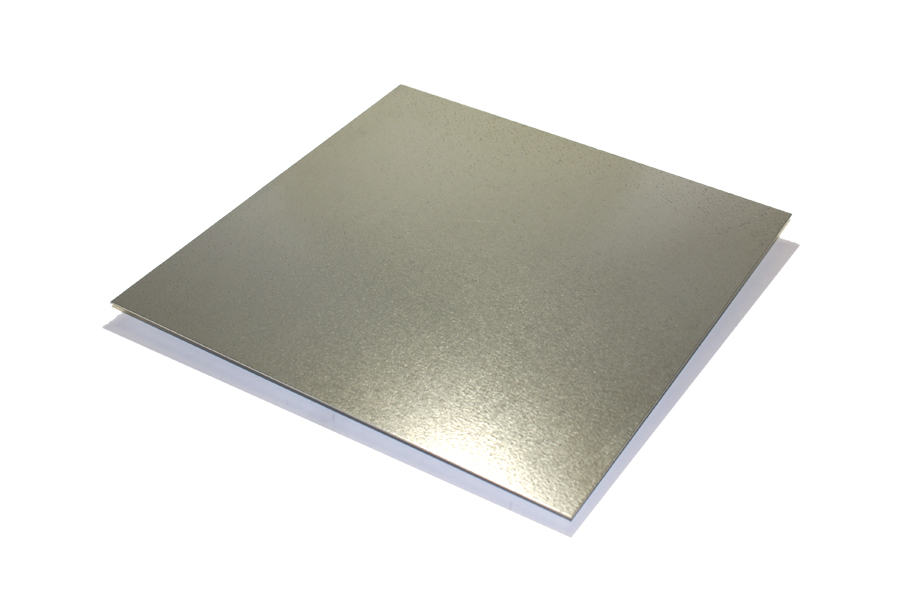
\includegraphics[width=5cm]{lamina.jpg}
\caption{A metal sheet}
\label{fig:2figsA}}
\qquad
\begin{minipage}{5cm}
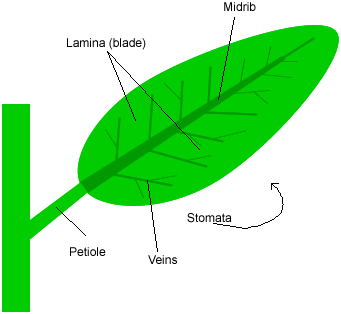
\includegraphics[width=5cm]{leaf.png}
\caption{a leaf}
\label{fig:2figsB}
\end{minipage}
\end{figure}



\subsection*{Finding the center of mass of a lamina}

The next goal is to be able to find the center of mass of the lamina, that is, the unique point with the property that once you apply a force to it, the lamina moves in the direction of the force without rotating. Another way to think about it is that you can balance the lamina on one finger, if your finger is touching it at its center of mass.

To see how to approach this, let's think of a simpler case first. Suppose that we have a rod without mass living on the real axis that has point mass $m_1$ attached to its left end, which is positioned at $x_1$ and a mass $m_2$ at its right end, positioned at $x_2$ and want to find the center of mass of the system, $a$. The position of $a$ would depend on both the masses and their distances from $a$, and indeed the correct  condition turns out to be $$m_1(a-x_1)=m_2(x_2-a),$$
or
$$ \sum_{i=1}^2m_i(x_i-a)=0.$$
\begin{figure}
\begin{center}
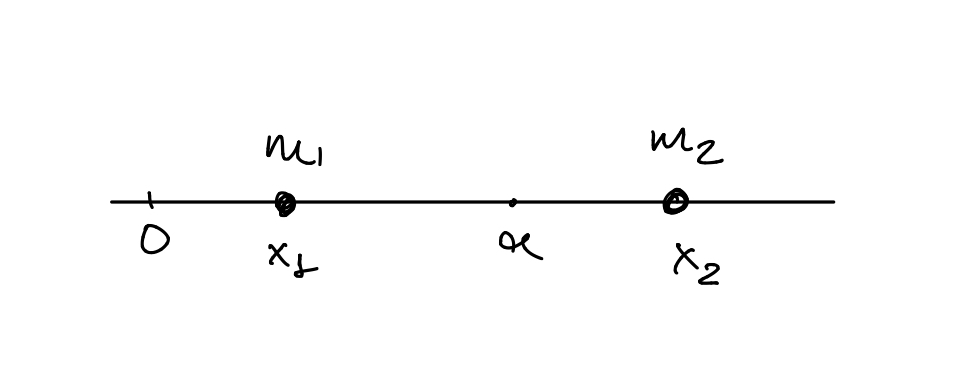
\includegraphics[scale=.2]{rod.jpg}
\caption{a rod with masses attached to it, on the real axis}
\end{center}

\end{figure}


It turns out that very analogous formulas are true for the $x$ and $y$ coordinates of the  center of mass $(\bar{x},\bar{y})$ of a lamina:
$$\iint_D \rho(x,y)(x-\bar{x}) dxdy= 0$$
and 
$$\iint_D \rho(x,y)(y-\bar{y}) dxdy = 0.$$
Solving for $\bar{x}$ and $\bar{y}$ in these formulas and using the expression we found before for the mass $M$, we find 
$$\bar{x}=\frac{1}{M}\iint_D x\rho(x,y)dxdy$$
and 
$$\bar{y}=\frac{1}{M}\iint_D y\rho(x,y)dxdy.$$

\begin{definition} Suppose we have a lamina occupying the domain $D$. We call the expression $$M_y:=\iint _D x\rho(x,y)dxdy$$ the \textbf{moment about the $y$ axis}.
We call the expression $$M_x:=\iint _D y\rho(x,y)dxdy$$ the \textbf{moment about the $x$ axis}.

With those definitions, the coordinates \textbf{center of mass} is given by $$(\bar{x},\bar{y})=(\frac{M_y}{M},\frac{M_x}{M}).$$
\end{definition}

Remark: A a lamina would be able to balance on a string placed on the line $x=\bar{x}$, and on a string placed on the line $y=\bar{y}$.

\vspace{.3 in}


\begin{example} Find the center of mass for a lamina occupying a half annulus $$D=\{(x,y):1\leq x^2+y^2\leq 4 \text{ and } y\geq 0\}$$ and having density function that is at each point inversely proportional to the cube of the distance of the point to the origin.
\end{example}
\begin{solution} The main difficulty here is to interpret the statement ``the density function that is at each point inversely proportional to the cube of the distance of the point to the origin''. Since the distance from the origin is given is given by $\sqrt{x^2+y^2}$, the statement means that there exists a number $k>0$ such that $$\rho(x,y)=\frac{k}{(x^2+y^2)^{3/2}}.$$
Note that this is an expression that can be easily rewritten in polar coordinates. The domain is written in polar coordinates as $D=\{(r,\theta) : 0\leq \theta\leq \pi, 1 \leq r\leq 2\}$ and therefore we have 

$$M=\iint_D \rho (x,y)dA=\int_0^\pi\int_1^2\frac{k}{r^3}rdrd\theta=\dots=k\frac{\pi}{2},$$

$$M_x=\iint_Dy \rho(x,y)dA=\int_0^\pi\int_1^2\frac{k}{r^3}(r\sin(\theta))rdrd\theta=\dots=k\log(4)$$ and


$$M_y=\iint_D x \rho(x,y)dA=\int_0^\pi\int_1^2\frac{k}{r^{3}}(r\cos(\theta))rdrd\theta=\dots=0.$$


This gives us for the coordinates of the center of mass $$(\bar{x},\bar{y})=(0,\frac{2\log(4)}{\pi}).$$ Note that the $k$ ends up not showing up in the expression of the center of mass!
\vspace{.1 in}

Remark: For $M_y$ you could argue by symmetry: the object's position is symmetric with respect to the $y$ axis and its density is also symmetric with respect to the $x$ axis, so it would 
be able to balance on the $y$ axis, that is, $\bar{x}=0$.
\end{solution}

\end{document}

